\documentclass[runningheads]{llncs}

% ---------------------------------------------------------------
% Include basic ECCV package
 
% TODO REVIEW: Insert your submission number below by replacing '*****'
% TODO FINAL: Comment out the following line for the camera-ready version
\usepackage[review,year=2024,ID=*****]{eccv}
% TODO FINAL: Un-comment the following line for the camera-ready version
%\usepackage{eccv}

% OPTIONAL: Un-comment the following line for a version which is easier to read
% on small portrait-orientation screens (e.g., mobile phones, or beside other windows)
%\usepackage[mobile]{eccv}


% ---------------------------------------------------------------
% Other packages

% Commonly used abbreviations (\eg, \ie, \etc, \cf, \etal, etc.)
\usepackage{eccvabbrv}

% Include other packages here, before hyperref.
\usepackage{graphicx}
\usepackage{booktabs}

% The "axessiblity" package can be found at: https://ctan.org/pkg/axessibility?lang=en
\usepackage[accsupp]{axessibility}  % Improves PDF readability for those with disabilities.


% ---------------------------------------------------------------
% Hyperref package

% It is strongly recommended to use hyperref, especially for the review version.
% Please disable hyperref *only* if you encounter grave issues.
% hyperref with option pagebackref eases the reviewers' job, but should be disabled for the final version.
%
% If you comment hyperref and then uncomment it, you should delete
% main.aux before re-running LaTeX.
% (Or just hit 'q' on the first LaTeX run, let it finish, and you
%  should be clear).

% TODO FINAL: Comment out the following line for the camera-ready version
\usepackage[pagebackref,breaklinks,colorlinks]{hyperref}
% TODO FINAL: Un-comment the following line for the camera-ready version
%\usepackage{hyperref}

% Support for ORCID icon
\usepackage{orcidlink}

\usepackage{cite}
\usepackage{multirow}
\usepackage{amsmath}
\begin{document}

% ---------------------------------------------------------------
% TODO REVIEW: Replace with your title
\title{Author Guidelines for ECCV Submission} 

% TODO REVIEW: If the paper title is too long for the running head, you can set
% an abbreviated paper title here. If not, comment out.
\titlerunning{Abbreviated paper title}

% TODO FINAL: Replace with your author list. 
% Include the authors' OCRID for the camera-ready version, if at all possible.
\author{First Author\inst{1}\orcidlink{0000-1111-2222-3333} \and
Second Author\inst{2,3}\orcidlink{1111-2222-3333-4444} \and
Third Author\inst{3}\orcidlink{2222--3333-4444-5555}}

% TODO FINAL: Replace with an abbreviated list of authors.
\authorrunning{F.~Author et al.}
% First names are abbreviated in the running head.
% If there are more than two authors, 'et al.' is used.

% TODO FINAL: Replace with your institution list.
\institute{Princeton University, Princeton NJ 08544, USA \and
Springer Heidelberg, Tiergartenstr.~17, 69121 Heidelberg, Germany
\email{lncs@springer.com}\\
\url{http://www.springer.com/gp/computer-science/lncs} \and
ABC Institute, Rupert-Karls-University Heidelberg, Heidelberg, Germany\\
\email{\{abc,lncs\}@uni-heidelberg.de}}

\maketitle


\begin{abstract}
  % 在图像领域,OCR中的STR一直是一个基础且热门的领域。随着语言模型的发展,由于STR任务同时涉及到图像和语言领域,越来越多的STR研究采用了文本与图像模型结合的多模态模型。本文中,我们提出了一种新型的文本图像结合模型,称之为文本编码输入模型。并且提出了一种针对性的训练方式,称之为循环迭代训练。在公开测试集上,我们的模型取得了SOTA的水平。并且我们通过实验证明,XInput模型可以有效的移植到任意STR模型中,均可以对比原模型具有较大的效果提升。
  Scene Text Recognition (STR) is a fundamental and popular area in imaging, particularly within Optical Character Recognition (OCR).	With language models advancing, the STR task, which encompasses both image and language domains, has seen a growing adoption of multimodal models combining text and images.	This paper introduces a novel integration method for text and images, named Text Encode Input (Xinput).	Experimentation has shown that the Xinput model can be effectively integrated into most STR models, significantly enhancing performance while maintaining model size and inference time.	The Xinput-based model achieved state-of-the-art performance on public test datasets.	
  \keywords{OCR \and STR \and multi-model}
\end{abstract}


\section{Introduction}
\label{sec:intro}

% 光学字符识别(OCR)是一项旨在将图像中的文本转换为可编辑文本的技术,广泛应用于数字化文档、自动化办公和信息检索等领域。与此同时,文本识别(Text Recognition,简称STR)是OCR领域中的一个重要分支,专注于识别和理解图像中的文本。相较于传统OCR系统,STR不仅仅局限于简单的字符检测和识别,而是致力于实现对文本的整体理解,包括布局、语义和上下文等方面的信息。
Optical Character Recognition (OCR) converts image-based text into editable format, extensively used in digitizing documents, automating offices, and retrieving information.	Meanwhile, Scene Text Recognition (STR) is a crucial OCR branch focusing on recognizing and understanding image-based text.	Unlike traditional OCR systems, STR goes beyond mere character detection and recognition to achieve comprehensive text understanding, including its layout, semantics, and context.	

% STR的应用已经深入到许多领域,如自动驾驶中的交通标志识别、图像检索系统中的图像标注、以及大规模文档数字化中的文本提取等。这使得STR在实际应用中扮演着关键的角色,为各行业提供了更高效、智能的文本处理解决方案。
STR's applications extend across multiple fields, including traffic sign recognition in autonomous driving, image annotation in retrieval systems, and text extraction in document digitization.	Consequently, STR plays a pivotal role in practical applications, offering more efficient and intelligent text processing solutions across industries.	

% 然而,尽管STR在实践中取得了显著的成就,它仍然面临着一系列挑战。其中之一是复杂场景下的文本识别,例如光照不均匀、遮挡、变形和多语言多字体等情况。这些挑战使得设计出稳健、通用的STR系统成为一个迫切而复杂的问题,需要深入研究和创新。
However, despite its significant achievements, STR still confronts numerous challenges.	One major challenge is recognizing text in complex conditions, including uneven lighting, occlusion, distortion, and diverse languages and fonts.	These challenges necessitate the design of robust and versatile STR systems, posing an urgent and complex issue demanding extensive research and innovation.	

% 在当前的研究趋势中,越来越多的学者将注意力集中在STR的改进和创新上,试图通过引入深度学习技术来提高文本识别的准确性和鲁棒性。这表明STR已经成为深度学习领域中备受关注的研究方向,吸引了众多研究者投入到其探索和推动中。
In current research trends, an increasing number of scholars are focusing on enhancing and innovating STR, aiming to boost text recognition's accuracy and robustness through deep learning techniques.	This highlights STR's emergence as a highly anticipated research area within deep learning, drawing numerous researchers to its exploration and advancement.	

% 最初在深度学习解决STR任务时,研究者们采用了多种单模态模型,其中一些已经成为领域内的经典代表。一种常见的方法是卷积神经网络(Convolutional Neural Network,CNN)与循环神经网络(Recurrent Neural Network,RNN)的结合而得到的CRNN(Convolutional Recurrent Neural Network)模型将CNN用于图像的特征提取,然后通过RNN处理提取的特征序列,最终实现对文本的识别。这种模型结构有效地捕捉了文本的时序信息,取得了在标准STR基准数据集上令人瞩目的性能。
Initially, to address STR tasks with deep learning, researchers utilized various unimodal models, many becoming classic benchmarks in the field.	A popular method is the CRNN\cite{shi2016end_CRNN} (Convolutional Recurrent Neural Network), which combines Convolutional Neural Network (CNN) and Recurrent Neural Network (RNN).	This model employs CNN for image feature extraction and RNN to process the extracted features for text recognition.	This structure effectively captures text's temporal information, achieving impressive performance on standard STR benchmarks.	

% 随着实际任务的逐渐复杂,传统的CRNN模型对于一些困难样本的识别难度很大。并且随着Attention机制的应用和Vision Transformer(ViT)的提出,研究者们在STR任务中探索了基于这些技术的新型模型。引入Attention机制的方法使得模型更加关注文本相关的区域,提高了对长文本和复杂场景的处理能力。Vision Transformer(ViT)则通过将图像划分为一系列块,并使用Transformer结构来处理这些块,成功应用于图像分类等领域。在STR任务中,ViT的引入为提高图像的全局理解能力提供了新的可能性。
As tasks grow increasingly complex, the traditional CRNN model struggles to recognize challenging samples.	The integration of the Attention\cite{vaswani2017attention} mechanism and the introduction of the Vision Transformer (ViT)\cite{dosovitskiy2020image_vit} have led researchers to explore innovative models for STR tasks.	The Attention mechanism enhances the model's focus on text-related areas, improving its processing of long texts and complex scenes,	Meanwhile, Vision Transformer (ViT) excels in tasks like image classification by segmenting images into blocks and employing the Transformer architecture for processing.	In STR tasks, ViT's adoption opens new avenues for enhancing image global understanding.	

% 在多模态研究方面,随着语言大模型的证明效果越来越有效,研究者们尝试将语言模型引入STR任务,以提升模型的性能。ABINet(Adaptive Bidirectional Integration Network)和TrOCR是两个具有代表性的多模态方法。ABINet通过自适应双向集成网络,有效融合了文本和图像信息,提高了文本识别的准确性和鲁棒性。TrOCR则采用了Transformer架构,将图像和文本信息结合,取得了在多个STR基准数据集上的优异性能,展现了多模态策略在STR中的潜力。这些研究丰富了STR模型的设计思路,为未来的深度学习研究提供了有益的启示。
In multimodal research, as linguistic models show increasing effectiveness, researchers are integrating these models into STR tasks to enhance performance\cite{li2023trocr,fang2021read_ABInet,fujitake2024dtrocr,zhao2023clip4str,ye2023ureader_llmocr,zeng2023large_llmocr,coquenet2023dan_llmocr}.	ABINet\cite{fang2021read_ABInet} (Adaptive Bidirectional Integration Network) and TrOCR\cite{li2023trocr} represent two key multimodal approaches.	ABINet, through its Adaptive Bidirectional Integration Network, effectively merges text and image information, enhancing text recognition's accuracy and robustness.	TrOCR employs the Transformer architecture to blend image and text information, achieving excellent performance across STR benchmarks, showcasing multimodal strategies' potential in STR.	These studies broaden the design concepts for STR models and offer valuable insights for future deep learning research.	

% 针对当前STR任务中的一些挑战和对已有模型的反思,我们提出了一种新的算法,采用编解码器结构实现文本与图像的多模态融合。与传统的复杂文本模型不同,我们的方法将文本信息直接与图像编码融合,作为编码器的输出传递给解码器。
Addressing challenges in current STR tasks and reflecting on existing models, we propose a novel algorithm for multimodal text-image fusion using a codec structure.	Unlike traditional complex text models, our method directly fuses text with image coding, passing it to the decoder as the encoder's output.	

% 我们决定放弃复杂文本模型的原因在于对自然环境下人类对文本的识别进行深入的观察。在很多情况下,人类对于文本的识别并不严重依赖于语言语义信息。特别是当一个熟悉所有字典字符的人面对需要识别的对象时,往往可以通过对比字典来准确地辨析出所有字符。这种观察特别在处理一些不符合传统语义排序的文本时更为显著。当需要识别的文本结果为"TYPO"时,了解语义的人可能会错误地将其纠正为"TYPE",而一个不了解语义但仅通过对比字典的人却能够正确识别。此外,文本图片通常在提供丰富信息协助识别时,语言模型的引入可能导致不必要的错误,例如将"TYPO"误纠正为"TYPE"。因此,我们得出结论:引入完整的语言模型可能不会明显提高识别准确率,或者说,如果通过引入语言模型获得了效果提升,那么应当有其他方法通过挖掘图像侧的信息获得相同的提升。
We decided to abandon complex text models based on thorough observations of how humans recognize text in natural settings.	Often, human text recognition does not heavily depend on linguistic semantics.	Specifically, a person familiar with dictionary characters can often accurately identify characters by comparison when faced with an object to recognize.	This observation becomes particularly significant with texts that deviate from traditional semantic order.	For example, with the text "TYPO", someone aware of semantics might mistakenly correct it to "TYPE", while someone comparing it to a dictionary without semantic understanding could identify it correctly.	Moreover, introducing a language model can introduce errors, like wrongly correcting "TYPO" to "TYPE", especially since textual images often offer ample clues for accurate recognition.	Therefore, we conclude that a full language model might not notably enhance recognition accuracy. If any improvement is seen, similar gains should be achievable by leveraging image-based information.	

% 我们提出的新算法在设计理念上汲取了传统学习方式的启发,并试图模拟人类学习的方式。传统学习通常是对图像是否包含某些字符进行初始猜测,损失函数通过判断猜测的正确性来进行纠正。与之相对比,人类学习识字的过程往往涉及到老师、家长或查阅字典的引导,通过对比字形的方式逐渐建立对字符的认知。即当小朋友认识一个全新的字符的时候,一般情况下是通过视觉获得字形信息的同时,有老师或者专业人士给出其读音,解释等字义信息。而不是等待小朋友进行猜测后再由专业人士判断是否猜测正确。
Our new algorithm is inspired by traditional learning methods, aiming to replicate human learning processes.	Traditional learning often starts with guessing whether an image contains specific characters, corrected through the loss function's assessment of accuracy.	In contrast, human learning to read and write typically involves guidance from teachers, parents, or dictionaries, and gradually builds character knowledge by shape comparison.	For instance, when learning a new character, a child visually learns its shape, while a teacher provides details on pronunciation, explanation, and meanings.	Unlike waiting for a child's guess to be judged by a professional, our algorithm directly presents textual information to the teacher or professional for immediate feedback.	

% 我们的新算法将文本信息直接编码输入到模型中,这相当于在模拟人类学习的方式。这一设计理念更符合人类识字的自然过程,通过对比字形的方式逐步建立对字符的认知。我们认为,将文本信息编码输入模型是一种对于这类引导的模拟,更贴合人类学习的方式,有望在文本识别任务中取得更好的效果。我们的新算法将注重在多模态融合中充分利用图像信息,以实现更为高效和鲁棒的文本识别。通过直接融合文本和图像的信息,我们在实验中验证这一新的设计理念所带来的性能提升。

Our new algorithm directly encodes text information into the model, simulating human learning processes.	This design aligns with the natural human literacy process, where knowledge of characters is built by comparing shapes.	We believe encoding textual information into the model simulates this guidance, closely mirroring human learning and potentially enhancing text recognition outcomes.	Our algorithm will leverage image information in multimodal fusion, aiming for more efficient and robust text recognition.	By fusing text and image information directly, we've experimentally validated the performance improvements of this design.	


\section{Related Word} \label{sec:relateword}
% 在过去的研究中,STR领域涌现了多种模型,其中一些代表性工作为我们新算法的设计提供了有益的参考。如卷积网络结构,代表为CRNN。基于注意力机制Transform结构,如ViTSTR, 引入语言模型的多模态模型结构,代表为ABINet。图.\ref{Fig:other_model_structure} 展示了几种常用的STR模型的简易结构对比。下面我们分别对这几种模型进行其特点介绍。
Past research in STR has produced a variety of models, with some serving as useful references for designing our new algorithms.	Representative models like the convolutional network structure (CRNN), the attention-based Transform structure (ViTSTR), and the multimodal model structure with a language model (ABINet) serve as valuable references for new algorithm design.	Fig.\ref{Fig:other_model_structure} illustrated the comparison between several common STR model sturture. Next, we will detail the characteristics of each model.	
\begin{figure*}
  \centering
  \includegraphics[scale=0.15]{./images/other_model_structure.eps}
  \caption{Search}     \label{Fig:other_model_structure}
  \end{figure*}

\subsection{Convolutional Neural Networks, CNN}
% 传统的卷积结构在STR中取得了显著的成果,其中CRNN(Convolutional Recurrent Neural Network)是一个典型代表。CRNN\cite{shi2016end_CRNN}通过卷积神经网络提取图像特征,然后通过循环神经网络对这些特征进行处理,实现了对文本的识别。这种结构在标准STR基准数据集上表现出色,但在处理长文本或复杂场景时仍然存在一些挑战。
Traditional convolutional structures, like the CRNN (Convolutional Recurrent Neural Network), have achieved significant results in STR.	The CRNN model extracts image features using a convolutional neural network and then processes these features with a recurrent neural network for text recognition.	While this structure excels in standard STR benchmarks, it faces challenges with long texts or complex scenes.

% 我们认为,CRNN已经可以看做一个编解码器结构,其中CNN是一个编码器,用以提取图片信息,而RNN则是用以处理编码信息的解码器结构。当然,受限于CNN与RNN本身的性能,其识别效果依然有较大的提升空间。主要性能限制有:序列信息衰减: RNN的一个主要问题是在处理长序列时,它可能会遇到梯度消失或梯度爆炸的问题。这意味着模型难以捕捉到序列中远离当前位置的信息。
We consider the CRNN as a codec structure, with CNN acting as an encoder to extract image information and RNN serving as a decoder to process this information.	However, due to the inherent limitations of CNN and RNN, there remains significant room for improvement in recognition performance.	The main limitation is sequence information decay: a significant issue with RNNs is their struggle with long sequences, potentially leading to gradient vanishing or explosion.	

% 有一些基于CRNN结构的优化,如MA-CRNN\cite{tong2020ma_MACRNN}, 增加了非对称卷积和特征重用网络,可以提取更丰富的语义信息,更好地处理上述挑战性条件,加入了注意机制,使模型充分融合了字符之间的上下文信息,从而更好地预测长文本。R2AM(带有注意力建模的递归循环神经网络)[17],GCRNN(门控循环卷积神经网络)[36]和Rosetta[4],还有一些如补充FPN,采用改进型的RNN(如长短时记忆网络,LSTM)和门控循环单元(GRU)等
Optimizations of the CRNN structure, like MA-CRNN\cite{tong2020ma_MACRNN}, enhance semantic information extraction and address challenges by adding asymmetric convolutional layers and feature reuse networks. These include integrating attention mechanisms for improved contextual understanding and long text prediction.	Other optimizations include R2AM\cite{lee2016recursive_R2AM}, GCRNN\cite{elbasani2021gcrnn}, and Rosetta\cite{borisyuk2018rosetta}, which utilize attention modeling, gated mechanisms, and complementary FPNs alongside enhanced RNNs, like LSTMs and GRUs, for improved text recognition capabilities.	

\subsection{Transformer-based Models} \label{subsec:transformer}
% ViTSTR(Vision Transformer for Scene Text Recognition)是一种基于Transformer架构的场景文本识别模型,ViTSTR的设计灵感来自于Vision Transformer(ViT),这是一种在计算机视觉领域取得显著成功的图像分类模型。ViT证明,仅使用transformer的encoder(好几个连起来)就可以实现ImageNet识别中得到SOTA结果。ViT继承了transformer的所有特性,包括速度和计算效率。ViTSTR与ViT之间的唯一区别是预测头。ViTSTR必须识别具有正确序列顺序和长度的多个字符,而不是单一对象类识别。在vitstr中,预测是并行进行的,显著的提升了推理速度。
ViTSTR\cite{atienza2021vision_VITSTR} (Vision Transformer for Scene Text Recognitio) is a scene text recognition model utilizing transformer architecture.	Inspired by the successful Vision Transformer (ViT) in image classification, ViTSTR adapts its principles for scene text recognition.	ViT demonstrated that state-of-the-art (SOTA) ImageNet recognition results could be achieved solely with the transformer's encoders in series.	ViT retains all transformer properties, including speed and computational efficiency.	Unlike recognizing a single object class, ViTSTR must identify multiple characters in the correct sequence and length.	Predictions are made in parallel in vitstr, which significantly increased the reasoning speed.	
% ViTSTR 体现了transform模型在STR领域的应用。这是一个完整的基于注意力机制的编解码器模型。体现了低参数量,低计算量的STR模型。主要是精度不变情况下的提速。并且模型精度也达到了当时的SOTA水平。
ViTSTR represents the application of transformer models in the STR domain.	It is a comprehensive codec model leveraging the attention mechanism.	It features a low-parameter, efficient computational design within the STR model framework.	Its main advantage is speed with maintained accuracy.	Additionally, the model's accuracy achieved state-of-the-art (SOTA) levels at that time.	

% ParSeq是此类基于Transformer架构的无额外引入预训练权重的SoTA模型。其特点为我们的方法Parseq使用置换语言建模学习了具有共同权重的内部AR LMS集合。使用Permuted Sequence modeling (PSM)技术,进一步优化了文本预测中各个字符间的关系。

ParSeq\cite{bautista2022parseq} is a state-of-the-art (SOTA) model utilizing Transformer architecture without relying on pre-trained weights.	ParSeq is characterized by learning a collection of internal autoregressive (AR) language models (LMS) with shared weights through substitution language modeling. The Permuted Sequence modeling (PSM) technique was used to further optimize the relationship between characters in text prediction. Specific details will be introduced later.

% 传统STR识别方式一般为按照顺序从左至右,从右至左,或两者结合的方式输出模型\cite{BTTR}。但是PARSeq作者指出,英文文本之间的字符信息与其左右字符并不是强相关的,而可以说是一种更为随机的关联。举例而言就是当识别“o”在“model”中时,按照从左到右识别的“m_”,与按照从右到左识别的“_del”均不太与“o”能形成语义关联,而是“m_de”这个固定词组可以与“o”形成较为直接的关联。依据此观点,PARSeq提出了Permuted Sequence modeling (PSM) 技术方案。PSM 使用了一个随机掩码$\mathcal{M}$ for attention operations to generate random dependency relationships betwwen the input context and the output.

Traditional STR recognition approaches output the model sequentially from left to right, right to left, or by combining both directions\cite{zhao2021handwritten_bttr}.	However, PARSeq's authors argue that the correlation of character information in English texts with their adjacent characters is not strong, but rather random.	For instance, when identifying "o" in "model", "m\_" (identified from left to right) differs from "\_del" (identified from right to left).	"\_del" is less likely to be semantically related to "o", whereas the fixed phrase "m\_de" has a more direct relation to "o".	Building on this concept, PARSeq introduces Permuted Sequence Modeling (PSM), employing a random mask $\mathcal{M}$ in attention operations to establish random dependencies between input contexts.	

% 根据ViTSTR和PARSeq的模型结构图,可以看出这两个模型也可以归类为编解码器结构。其二者的编码器均为VIT-encoder。 解码器部分ViTSTR采用了全连接层契合最终输出结构。而PARSeq采用了Transform-decoder结构,并且进行了一定的优化。
The model structure diagrams for ViTSTR and PARSeq reveal that both models fit the codec structure category.	Both models feature a VIT-encoder as their encoding component.	ViTSTR's decoder incorporates a fully connected layer to fit the final output.	Meanwhile, PARSeq employs an optimized Transform-decoder structure.	

\subsection{Vision-Language Models} \label{subsec:vision-language}
% 多模态模型在场景文本识别(Scene Text Recognition, STR)领域的应用已经引起了广泛关注。文本和图像之间的丰富关联性使得整合文本和图像信息成为提升场景文本识别性能的有效途径。其中,文本图像多模态模型作为一种创新的方法,不仅综合了文本的语义信息,还利用了图像中的上下文和视觉特征。 在这些多模态模型中,文本嵌入和图像特征通常通过融合层进行整合,使得模型能够同时考虑文本和图像的语义信息。注意力机制被广泛应用,以使模型能够动态地关注图像中与文本相关的区域,提高文本检测和识别的准确性。
Multimodal models have gained significant attention in Scene Text Recognition (STR) due to their application.	Integrating text and image information, given their rich correlation, effectively enhances scene text recognition performance.	Text-image multimodal models, an innovative approach, integrate both semantic text information and contextual, visual features from images.	In multimodal models, a fusion layer typically integrates text embeddings and image features, allowing the model to process semantic information from both sources.	Attention mechanisms enable models to dynamically focus on text-relevant image regions, enhancing text detection and recognition accuracy.	

% ABINet是一个著名的采用语言图像多模态结构的STR模型,ABINet在视觉模型和语言模型之间阻断梯度流,以实现语言的显式建模。其次,提出了一种基于双向特征表示的双向完形填空网络(BCN)语言模型。最后,提出了一种语言模型迭代修正的执行方式,有效地缓解了噪声输入的影响,可以总结为首先输入图像到视觉模型,提取图像特征以及输出预测结果;将视觉模型的预测结果送入语言模型来提取语言特征并预测结果;将视觉模型的视觉特征和语言模型的语言特征进行融合来得到融合的预测结果;融合的预测结果再送入语言模型,迭代地进行细化,以得到最终的预测结果。
ABINet, a prominent STR model, utilizes a multimodal structure for language images, blocking gradient flow between visual and linguistic models to explicitly model language.	It introduces a Bi-directional Completion Network (BCN) language model based on bi-directional feature representation.	Additionally, it proposes iterative correction of the language model to mitigate noisy input effectively.	The network structure involves: inputting images to the visual model to extract features and predict outcomes; using these predictions to derive linguistic features and further predictions in the language model; combining visual and linguistic features for enhanced predictions; and iteratively refining these combined predictions in the language model to achieve final outcomes.	

% 当然,多模态模型也可以被归纳为编解码器结构,其编码器部分除了图片编码器也有文本编码器。并且编解码器之间有不同的链接方式。图展示了几种的多模态模型结构。
The multimodal model can be summarized as encoder-decoder structure,	This structure includes both text and image encoders in the encoding part.	
% Additionally, there are various methods for linking codecs.	The figure demonstrates several structures of multimodal models.	
\subsection{with LLM Models} \label{subsec:LLM}
% 随着large language models(LLM)被证明有着显著的效果,语言大模型也越来越多的使用在STR模型中。语言大模型在STR中的应用,一方面体现在其对于上下文信息的强大建模能力。通过在大规模语料上进行预训练,语言大模型能够学习到深层次的语言表示,更好地理解词汇之间的关系和语境。这种能力在处理具有丰富语义信息的文本时显得尤为重要,例如处理包含多义词、专业术语或特定领域语境的文本。
Given the proven significant effects of Large Language Models (LLMs), their use in STR modelling is increasing.	The application of large language models in STR notably enhances the modeling of contextual information.	Through pre-training on extensive corpora, these models learn profound linguistic representations, enabling a deeper understanding of word-context relationships.	This capability is crucial for processing texts rich in semantic information, including those with polysemous words, specialized terminology, or domain-specific contexts.	

%另一方面,语言大模型的引入在一定程度上弥补了传统STR模型对于语义信息的不足。传统模型在字符级别进行识别,对于整体语义的理解相对较弱,而语言大模型的引入使得STR模型能够更好地理解文本的语义内容,提高对于复杂场景和长文本的识别能力。
Additionally, the use of large language models addresses the semantic limitations of traditional STR models to some extent.	whereas incorporating linguistic models enhances the STR model's understanding of text semantics and its ability to recognize complex scenes and lengthy texts.	

% TrOCR, Clip4STR与DtrOCR是一些著名的结合语言大模型的STR模型,并且均达到了SOTA水平。其中TrOCR使用使用RoBERTa(Liu等人2019)模型和MiniLM(Wang等人2020b)模型来初始化解码器,Clip4STR使用Clip来初始化模型,DtrOCR采用gpt2作为解码器。其中TrOCR和Clip4STR均为较为明显的编解码结构。而DtrOCR可以认为为编码器为一个线性切块处理的简单模型,而解码器为gpt2结构的编解码器模型。
TrOCR, Clip4STR, and DtrOCR are well-known STR models that combine large language models and achieve the state-of-the-art (SOTA) level.	TrOCR initializes its decoder using the RoBERTa (Liu et al. 2019) and MiniLM (Wang et al. 2020b) models,	Clip4STR uses Clip to initialize the model, whereas DtrOCR employs GPT-2 as its decoder.	TrOCR and Clip4STR exhibit more apparent codec structures.	Conversely, DtrOCR can be considered a simpler model, with its encoder performing linear chunking and its decoder based on a GPT-2 codec structure.	

% 值得注意的是,语言模型的引入会导致模型参数量与训练难度的急剧上升。并且由于语言模型是采用预训练的形式引入STR模型,其训练样本量显著高于传统STR模型的训练样本量。所以通过语言模型结合获得的更高的STR准确率指标,一定程度上并不能直接证明是模型结构的优化,而是有可能是由于更多的训练样本所导致的。
The introduction of the language model significantly increases the number of model parameters and the difficulty of training.	Furthermore, because the language model is integrated through pre-training, the STR model requires a much larger training sample size than traditional STR models.	Therefore, the improved STR accuracy metrics achieved by integrating language models do not directly prove structural optimization but may result from the larger training sample size.	

\section{Method} \label{sec:method}
% 我们提出的Xinput训练方式是一种通用训练方式,可以应用在任何现有的文本识别模型中。PARSeq作为现有的无额外引入预训练模型的SOTA模型,是作为证明xinput方案可以进一步提升模型效果的最佳样例。在介绍xinput之前,我们首先介绍一下PARSeq和permuted sequence modeling (PSM)。我们将后续介绍parseq结合xinput的模型parseq-xi。同时我们也会简略介绍下VITSTR, 和其与xinput结合的VITSTR-Xi。
We propose the Xinput training approach as a universal method applicable to all existing text recognition models.	PARSeq, an existing state-of-the-art (SOTA) model that does not require pre-trained models, serves as an ideal example to demonstrate how the Xinput scheme can enhance model performance.	Before delving into Xinput, we first explore PARSeq and permuted sequence modeling (PSM).	Next, we introduce PARSeq-Xi, which merges PARSeq with Xinput, and briefly cover VITSTR and VITSTR-Xi, integrating VITSTR with Xinput.	

\subsection{Xinput} \label{subsec:xinput}
% 通过之前的分析,可以认为现阶段的大部分STR模型均可以看为一个编解码结构。我们认为,将文本信息补充进入编码器输出提供给解码器是一种更符合人类学习习惯的做法,我们将其称之为text input(Xinput)。这个做法可以插在任意编解码器结构中。并且这种做法对于模型编解码器均有有效的提升。图./reff{Fig:xinput}展示了xinput的基本流程。
Based on prior analyses, it can be argued that most current STR models resemble a codec structure.	We propose enhancing the codec structure by incorporating text information into the encoder output for the decoder, a method we refer to as text input(Xinput). This can be integrated into any codec structure, shown in Fig./ref{Fig:xinput}, 

\begin{figure*}
  \centering
  \includegraphics[scale=0.15]{./images/xinput_structure.eps}
  \caption{
    % Xinput 的基本结构和训练推理过程。受限于篇幅省略了编解码器的具体步骤。其中Image Pre-Processing包括了图片预处理,归一化等步骤。Dict Encoding 中文本转换为编码,Text Pre-Processing将文本编码进行处理,包括组batch,one-hot embedding等,Zero-Padding为补零操作,目的为尺寸对齐图像编码器的输出,其输出尺寸应为$bs \times max_length \times image_embedding_size$,其中bs代表batch-size, max_length代表文本最大尺寸, image_embedding_size代表图像编码器的embedding size参数。Merge部分代表将文本编码与图像编码相结合。组成新的编码输入后续解码器中。
    Xinput architecture and training/inference overview. Details for the Encoder/Decoder layers are omitted due to space constraints. Image Pre-Processing includes image preprocessing, normalization and other steps. Dict Encoding converts the Text to encoding. Text Pre-Processing processes the text encoding, including the group batch and one-hot embedding. Zero-Padding is the zero-complement operation to size align the output of the image encoder. The output size should be $bs \times max\_length \times image\_embedding\_size$, $bs$ indicates batch-size, $max\_length$ indicates the maximum text size, and $image\_embedding\_size$ indicates the embedding size parameter of the image encoder. The Merge part stands for combining text encoding with image encoding. Compose a new encoding into the subsequent decoder.}
  \label{Fig:xinput}
  \end{figure*}


% 编码器的作用是从$H\timesW\timesC$的图像矩阵信息中,提取出图像内在信息,并提供给解码器获取希望的输出。在STR模型完美情况下,编码器应当提取完备的文字信息并忽略任何背景,干扰,形变所带来的错误信息。解码器可以将完备的图片信息准确的转换为文本信息。而模型初始化,当无预训练模型介入时,编码器并不能提供任何有效信息给解码器,同时解码器也不会反向回传有效的信息。当然,设计好的超参可以保证模型很快的收敛,并且开始有效的信息传递。但是此时并不能保证所有的干扰信息均被剔除。而且极大概率由于大部分数据中并不存在干扰信息,一些较难样本的干扰信息会被保留并且被编码器编码后输出至解码器。被解码器作为是有效信息而进行训练。
The encoder's role is to extract intrinsic information from the $H\times W\times C$ image matrix and provide it to the decoder to achieve the desired output.	In an ideal STR model scenario, the encoder should extract complete textual information and disregard errors caused by background, interference, and distortion.	The decoder should accurately convert complete picture information into text.	During model initialization, without a pre-trained model, the encoder fails to provide valid information to the decoder, which in turn cannot return valid information.	Well-designed hyperparameters can ensure rapid model convergence and the start of valid information delivery.	However, it's not guaranteed that all interference will be eliminated.	Given that most data lacks interference, there's a high chance that some challenging interference samples will be retained, encoded by the encoder, and passed to the decoder.	The decoder treats these samples as valid information.	
% 而引入文本信息对模型训练的初始化,中间过程和最终过程均会有一定的提升。初始化时,图像编码分支的信息是混沌且无效的,此时引入完备的文本信息可以使解码器进行有效的训练。此时解码器的工作可以看做复制引入的文本信息。为了方便展示,我们默认不考虑batch维度。我们将文本信息记为$X = {x_1, x_2, ..x_n}$, 经过文本编码和拓展后,可以得到文本编码信息$\textbf{X}_{input}\in\mathbb{D}^{L_{t}\times E}$。其中$\mathbb{D}$代表对文本信息进行编码的编码空间;。$L_{t}$代表文本长度; $E$代表为了与图片编码信息拼接而进行尺寸转换后的文本尺寸信息。Eq.{eq:begin}展示了初始化阶段的模型训练流程。

Introducing textual information enhances the initial, intermediate, and final stages of model training.	During initialization, the image coding branch contains chaotic and invalid information; introducing complete textual information enables efficient decoder training.	At this stage, the decoder's task can be seen as replicating the introduced textual information.	For simplicity, we omit the batch dimension by default.	We represent textual information as $X = {x_1, x_2, \ldots, x_n}$. After encoding and expanding the text, we obtain the encoded text information $\textbf{X}_{input}\in\mathbb{D}^{L_{t}\times E}$.	Where $\mathbb{D}$represents the encoding space for encoding text information; . $L_{t}$represents the text length; $E$represents the text size information converted to concatenate the image encoding information. Eq.{eq:begin} shows the model training process in the initialization phase.

\begin{equation}\label{eq:begin}
    \textbf{y} = \textit{T}^{-1}(\textbf{X}_{input}) = \textit{Decoder}(\textit{Encoder}(img) | \textbf{X}_{input}  )
\end{equation}

% 其中$y$代表预测输出,$\textit{T}^{-1}(\textbf{X}_{input})$代表对文本编码输入的逆运算; $\textit{Decoder}$ 代表解码器运算,$(\textit{Encoder}(img)$代表图像编码运算,$|$代表图像编码信息和文本编码信息进行拼接
Where $y$ represent forecast the output, $\textit {T}^{-1} (\textbf {X}_{input}) $on behalf of the inverse operation of text encoding input; $\textit{Decoder}$ represents decoder operation, $\textit {Encoder}(img)$represents image coding operation, and $|$represents the stitching of image coding information and text coding information.

% 可以看出,初始化阶段,由于完备的$\textbf{X}_{input}$输入,图片文本编码器部分可以认为是噪音输入,而解码器退化为学习最终结果输出的逆过程,即学习$\textit{T}^{-1}()$。在文本编码操作均是可逆操作,CTC中即退化为全等,或Transform中的硬编码embeding. 我们认为这种学习是较为方便的。
During the initialisation phase, with the complete $\textbf{X}_{input}$, the image text encoder is seen as introducing noisy input. Meanwhile, the decoder simplifies into learning the output's inverse process, which is learning for the $\textit{T}^{-1}()$. All the operater for text input is inversible, where the operat is becoming fully equivalent in CTC or hard-coded embedding in Transform.	We consider this learning approach to be more convenient.	

% 当模型训练到一定程度时,其已经有较为明显的收敛,此时模型编码器部分可以认为暂时是无有效信息提取的。解码器部分应可以较为可靠的从文本编码处得到较为准确的输出。此时应逐步将图像编码信息引入解码器:Eq.{eq:begin} 转换为 Eq.{eq:inter}。
Once the model is sufficiently trained and has significantly converged, the encoder may temporarily lack effective information extraction capabilities.	The decoder should then be capable of deriving more accurate outputs from the text encoding.	Consequently, image encoding information should be gradually integrated into the decoder, transitioning from Eq.{eq:begin} to Eq.{eq:inter}.	
\begin{equation}\label{eq:inter}
    \textbf{y} = \textit{T}^{-1}(\textbf{X}_{input}) = \textit{Decoder}(\textit{Encoder}(img) | (\textbf{X}_{input} \cdot \mathbb{M} + pad_{id} \times ( \textbf{1} - \mathbb{M} )) )
\end{equation}

% 其中$\mathbb{M}$是尺寸同$\textbf{X}_{input}$的随机0,1掩码。$pad_id$代表文本编码中的填充符号。
where $\mathbb{M}$ represents a random 0,1 mask matching the size of $\textbf{X}_{input}$; $pad_id$ present padding tokens.

%Eq.{eq:inter}中表示使用掩码掩盖一部分文本信息,并使用填充信息补充被掩盖的信息后与图像信息拼接输入解码器模块。此时明显的是,由于被掩盖了一部分文本信息,初始阶段解码器模型并不能正确的得到预计的输出y。此时缺失的信息模型只能从图像编码部分获取。即模型逐步从文本信息侧转移到图片信息侧。
Eq.{eq:inter} indicates that a portion of the text information is masked and then supplemented with filler information before being combined with image information for input into the decoder module.	Consequently, due to the masked text information, the initial stage of the decoder model fails to accurately produce the expected output y.	The missing information can only be sourced from the image encoding part at this stage.Thus, the model gradually transitions from relying on textual to image information.

%掩码设计中,关键在于选取合适的保留文本的随机阈值ratio信息是关键的一步。在Xinput中,我们采用结合上一个batch的loss的方式来确定本batch的ratio, 如Eq.\ref*{eq:ratio}
The crucial aspect of batch design involves selecting an appropriate random threshold ratio to retain the text information.	In Xinput, the ratio for the current batch is determined by considering the loss from the previous batch.	

\begin{equation}\label{eq:ratio}
    ratio = \alpha \cdot (Loss - \beta)
\end{equation}

%其中$\ratio$代表随机掩码的随机率,ratio越高,掩码中的1越多,保留的文本信息越多,反之保留的文本信息越少。$\alpha$ 与 $\beta$ 分别是一个浮点数,将损失值$Loss$与ratio关联。$Loss$代表上一个batch经过模型后得到的损失数值。
Where $ratio$ represents the randomness rate of the random mask. The higher the ratio, the more 1 in the mask, the more text information is retained; otherwise, the less text information is retained. $\alpha$and $\beta$are floating-point numbers that relate the Loss value $Loss$to the ratio. $Loss$Indicates the loss value of the last batch after the model.

% 使用损失值确定ratio可以自动化的从初始化部分过度到中间训练部分以及后续的最终部分。当loss较高时,表明模型没有收敛,此时应使用较高的ratio。随着loss的降低,表明模型已经可以逐步提取有效信息,可以适当降低ratio,使模型更多的从图像侧提取信息。ratio降低后由于缺失文本侧信息,loss会有一定的回溯,但由于已经从图像侧获取的信息补充,loss回溯幅度应低于之前,可以保证模型一直收敛。
Automating the ratio determination based on the loss value allows for a seamless transition from initialization to intermediate training and finally to the concluding part.	A high loss indicates the model has not yet converged, necessitating a higher ratio.	Decreasing loss suggests the model is gradually extracting valid information, allowing for a reduction in the ratio to encourage more information extraction from the image side.	After reducing the loss, some backtracking may occur due to insufficient text information. However, thanks to the information gained from the image side, the loss should be lower than before, indicating ongoing model convergence.	Moreover, the information acquired from the image side should result in a lower loss backtracking amplitude than previously, ensuring continuous model convergence.	

%当loss收敛到低于 $\beta$ 时,文本侧已经不会提供信息,模型应以可以完全从图像侧获取信息,即成为Eq.\cite{eq:end}形式。若出现困难样本导致loss上升后,模型会重新从文本侧获取信息,引导模型继续训练,即回退为Eq.\cite{eq:inter}形式。
Once the loss converges below the threshold $\beta $, the text side ceases to provide information, allowing the model to fully extract information from the image side, transitioning to the form described in Eq.\cite{eq:end}.	Should difficult samples increase the loss, the model will revert to sourcing information from the text side to facilitate continued training, reverting to the form outlined in Eq.\cite{eq:inter}.	

\begin{equation}\label{eq:end}
    \textbf{y} = \textit{T}^{-1}(\textbf{X}_{input}) = \textit{Decoder}(\textit{Encoder}(img) | pad_{id} \cdot \textbf{1})
\end{equation}

% 可以看出,当模型loss稳定低于$\beta$数值时,补充xinput方式的STR模型基本退化为原基于编解码器结构的模型结构。并且在推理过程中,文本侧也不提供额外的信息。即最差情况下, 补充xinput方式的STR模型效果应当与原STR模型效果持平。
It can be seen that when the model loss is stable below the value of $\beta$, the STR model supplemented with xinput mode basically degenerates to the original model structure based on codec structure. And during the reasoning process, the text side does not provide additional information. That is, in the worst case, a STR model supplemented with xinput should have the same effect as the original STR model.

\subsection{Xinput with SOTA models}

% 如之前所说,xinput方式可以补充到任意基于编解码器结构的STR模型中,并且最差情景下效果应不低于原STR模型。本文我们主要对比了两种STR模型结合Xinput方式的效果:vitstr与parseq。在原始的vitstr使用的是在encoder后直接使用全连接层层作为编码最终输出。并且输出结果是一个embeding结构,$y\in R^{B\times S\timesNC}$, 其中$B$是batch size, $S$是seqlen, $NC$是字典长度。即输出的内容中$y[b][s][nc]$的数值代表在第$b$batch中,第$s$个字符是$nc$的可能性。在最终输出时提取每一个位置中最大可能性的字典内容。根据之前的分析,当在text pre-processing中对文本输入进行one-hot embedding操作后,模型训练的初始阶段的全连接层的期待学习为直接映射,即$\textit{T}^{-1} = \mathbf{I}$, 其中$\mathbf{I}$代表单位矩阵。显而易见的是,这个学习应当是简单且迅速的。

As mentioned earlier, the xinput approach can be added to any STR model based on the codec structure, and the worst-case scenario should be no less effective than the original STR model. In this article, we mainly compare the effect of Xinput on two STR models: vitstr and parseq. The original vitstr uses the full connection layer directly after the encoder as the final output of the encoding. And the output result is a embedding structure, $y\in R^{B\times S\times NC}$, where $B$ is batch size, $S$ is sequence length, $NC$ is dictionary length. That is, the value of $y[b][s][nc]$ in the output represents the possibility that the $s$ character is $nc$ in the $b$ batch. The maximum possible dictionary content in each location is extracted at the final output. According to the previous analysis, when the one-hot embedding operation is on text input in text pre-processing, the expected learning of the full connection layer in the initial stage of model training is direct mapping, that is, $\textit{T}^{-1} = \mathbf{I}$, where $\mathbf{I}$ represents the identity matrix. Obviously, this learning should be easy and quick.

%Parseq 采用Transform-decoder结构的作为解码器。Text pre-processing过程中,既可以采用相同与vitstr方式的进行one-hot embedding编码方式,也可以采用同语言模型的token输入方式。基于之前的研究\cite{}, 两者当完全输入的时候,Transform结构均可以完成复现学习。
Parseq uses the Transform-decoder structure as the decoder. In the Text pre-processing process, the coding mode of the one-hot embedding is the same as that of vitstr, or the token input mode of the same language model. Based on the previous study \cite{}, the Transform structure can complete repeat learning when both are fully input.

% 另外值得说明的是,如之前分析,CRNN 固然也可以分为编解码器结构,即CNN作为图片编码,RNN作为解码。故而CRNN模型结构也是可以与Xinput方式相结合的。但是由于RNN的时序输入特性,图片特征结合文本特征后,显然理论上并不能对于RNN的反向传播训练起优化作用。故而我们也没有再具体介绍CRNN与Xinput结合的模型结构。
In addition, it is worth explaining that, as previously analyzed, CRNN can indeed be categorized into a codec structure, with CNN for image encoding and RNN for decoding.	Thus, the CRNN model can also integrate the Xinput approach.	However, the temporal input nature of RNNs means that theoretically, combining image and text features does not optimize RNN's backpropagation training.	Consequently, we do not present a model structure that combines CRNN with Xinput.	

\subsection{Xinput with LLM models}
% 另外与LLM结合的STR模型由于其也可以归纳为编解码结构,故而也可以与我们提出的Xinput方式相结合。但是由于其他结合语言模型的STR模型均采用了预训练的语言模型,如之前所说,采用不同的预训练语言模型对最终STR模型的准确率指标会有较大的影响。后续我们没有再具体评估此类模型结合xinput后的的效果。
The STR model, when combined with LLM, can also adopt our proposed Xinput approach, as it fits well with coding and decoding structures. However, as all other STR models integrating language models utilize pre-trained language models, the choice of these pre-trained models significantly influences the final STR model's accuracy metrics.	We have not specifically assessed the impact of combining these models with Xinput in subsequent evaluations.	

\section{Experiment}
\subsection{Dataset}
% 和之前的工作\cite{parseq}相同,我们采用了和经典STR模型相同的合成数据集:MJSynth (MJ)[18](MJ,9M samples) 和SynthText (ST)[19](ST, 6.9M samples). 另外 we use COCO-Text (COCO) [70], RCTW17 [62], Uber-Text (Uber) [84], ArT [16], LSVT [65], MLT19 [52], and ReCTS [83]. A comprehensive discussion about these datasets is available in Baek et al. [4]. In addition, we also use two recent large-scale real datasets based on Open Images [35]: TextOCR [63] and annotations from the OpenVINO toolkit [36]. 训练数据的数据处理方式和增强方式同\cite{parseq}. 
Following previous work \cite{baek2021if_TRBA_discuss,bautista2022parseq}, we utilize the same synthetic datasets as traditional STR models: MJSynth (MJ) \cite{jaderberg2014synthetic_MJ} with 9M samples and SynthText (ST) \cite{gupta2016synthetic_ST} with 6.9M samples.	Additionally, we employ COCO-Text (COCO) \cite{veit2016coco_Coco}, RCTW17 \cite{shi2017icdar2017_RCTW17}, Uber-Text (Uber) \cite{zhang2017uber_Uber}, ArT \cite{chng2019icdar2019_art}, LSVT \cite{sun2019icdar_LSVT}, MLT19 \cite{nayef2019icdar2019_MLT19}, and ReCTS \cite{zhang2019icdar_ReCTS}.	A comprehensive discussion on these datasets is available in Baek et al \cite{baek2021if_TRBA_discuss}.	Furthermore, we utilized two recent large-scale real datasets based on Open Image \cite{krasin2017openimages_openimages}: TextOCR \cite{singh2021textocr_TextOCR} and annotations from the OpenVINO toolkit \cite{krylov2021open_openvino}.

% 为保证测试效果,依据之前的工作[8],我们使用IIIT 5k-word (IIIT5k)[20],CUTE80 (CUTE)[21],Street View Text (SVT)[22],SVT-Perspective (SVTP)[23],ICDAR 2013 (IC13)[24]和ICDAR 2015 (IC15)[25]作为评估的数据集。我们使用Long和Yao [26]对IIIT5k,CUTE,SVT和SVTP进行大小写敏感的注释。请注意,IC13和IC15在文献中常用的各自测试集分为两个版本——IC13有857和1,015;IC15有1,811和2,077。为避免混淆,我们将基准称为IIIT5k、CUTE、SVT、SVTP、IC13(1,015)和IC15(2,077)的联合。这六个基准数据集仅有总共7,672个测试样本,称之为all测试集,而使用IC13(857)和IC15(1811)的数据集称之为clean测试集。
For testing, based on prior studies, we utilize IIIT 5k-word (IIIT5k) \cite{mishra2012scene_iii5k}, CUTE80 (CUTE) \cite{risnumawan2014robust_cute80}, Street View Text (SVT) \cite{wang2011end_SVt}, SVT-Perspective (SVTP) \cite{phan2013recognizing_svtp}, ICDAR 2013 (IC13) \cite{karatzas2013icdar_IC13}, and ICDAR 2015 (IC15) \cite{karatzas2015icdar_IC15} for evaluation.	Case-sensitive annotations for IIIT5k, CUTE, SVT, and SVTP are based on Long and Yao \cite{long2020unrealtext_sensitive4test}.	It is noted that IC13 and IC15 often appear in two versions in literature - with IC13 having 857 and 1,015 test samples, and IC15 having 1,811 and 2,077 samples.	To avoid confusion, we collectively refer to these benchmarks as IIIT5k, CUTE, SVT, SVTP, IC13(1,015), and IC15(2,077).	The six benchmark datasets collectively contain 7,672 test samples, termed the ALL test set, while the versions with IC13 (857) and IC15 (1,811) samples are known as the CLEAN test set.	

\subsection{experimental details}
\subsubsection{Xinput variants}
% xinput结构拼接在广义编码器所获取的图像编码后。其尺寸尺寸为$\textbf{X}_{input}\in\mathbb{Q}^{bs\timesC\timesS}$, 其中$bs$与$C$代表图像编码的batch-size 与 Channel-size, 其数值与不同拼接的编码器相关。$S$代表的是固定的文本编码长度。其数值与标注数据有关。在STR英文单词识别情景下,本文中的$S$若无特殊说明,固定设置为36。
The Xinput structure is integrated following the image encoding phase of the generalized encoder.	The size of $\textbf{X}_{input}$ is defined as $\in\mathbb{Q}^{bs\times C\times S}$, where $bs$ and $C$ denote the batch size and channel size of the image encoding, respectively, and their values vary according to the encoder used.	$S$ represents the fixed length of text encoding.	Its value depends on the labeled data.	For STR English word recognition, $S$ is set to 36 in this study, unless noted otherwise.	

% xinput的文本内容会根据模型训练中的loss数值进行动态掩码,如Eq.\cite{eq:ratio}所示。由于不同的数据集,损失函数,模型的结构,超参设置等均会对模型训练中的损失函数产生影响。所以若采用固定的$\alpha$或$\beta$数值对不同的模型是不合理的。本文中,我们采用如下方式设置相关参数。首先采用无xinput的方式训练模型至模型稳定,记录稳定的loss值与达到稳定态的轮次。当模型达到稳定态的轮次较快时,设置较小的$\alpha$,使模型训练中可以更快的减少来自文本侧的信息。反之则设置较大的$\alpha$,使模型训练中保留更多的文本信息进行协助。同时设置$\beta \leq loss / \alpha$, 保证模型可以在后期达到稳定后,$ratio \le 0$, 使文本侧信息被完全屏蔽。
Xinput's text content is dynamically masked based on the model training's loss values, as demonstrated in Eq.\cite{eq:ratio}.	Various factors such as datasets, loss functions, model structures, and hyperparameter settings impact the loss function during model training.	Therefore, using fixed $\alpha$ or $\beta$ values for different models is not advisable.	This paper outlines the following method for setting relevant parameters.	First, we train the model without Xinput until it stabilizes, recording the stable loss value and the number of rounds to achieve this state.	If the model stabilizes quickly, we set a smaller $\alpha$ to accelerate the reduction of text information during training.	Conversely, we set a larger $\alpha$ to retain more textual information for training assistance.	Simultaneously, we set $\beta \leq loss / \alpha$ to ensure model stabilization at later stages, with $ratio \le 0$, blocking text information completely.	

\subsubsection{Other variants} 
%对于不涉及Xinput的其他参数,除训练最大轮次外,我们采用\cite{Parseq}所设置的parseq, crnn, vitstr模型的最优参数作为我们的基础参数进行训练。后续结果展示中如果有不同的参数会进行说行。由于我们补充了文本信息,模型收敛到稳定所需的轮次会更多。实验中,我们根据模型训练过程中的loss曲线确定其最终的轮次。同样作为对比组,其他模型也会训练到相对应的轮次。
For parameters unrelated to Xinput, we adopt the optimal settings for PARSeq, CRNN, and VITSTR models as outlined in \cite{bautista2022parseq}, with the exception of the maximum training epoches.	In subsequent result presentations, any deviations in parameters will be noted.	Adding text information increases the number of epoches needed for model convergence and stabilization.	In our experiments, the final number of training epoches is determined by the model's loss curve.	For comparison, other models are trained for an equivalent number of epoches.	

\subsubsection{Hardware and Software}
% 实验环境为双卡V100, Cuda V11.7, python3.9.18, pytorch2.1.2, 其他具体可参考:Github
The experimental setup includes a dual V100 GPU configuration, Cuda V11.7, Python 3.9.18, and PyTorch 2.1.2. Additional details can be found on GitHub.	

\subsection{comparison of State-of-the-art}
% we compare the xinputs methods with previous SOTA methods which 不引入外部预训练模型 on 8 common STR bencharks in Table.\ref{table:Synres}. The xinputs methods 对于原始模型均有有效的提升,并且xinput+parseq也超越了原有的SOTA效果。 
In Table.\ref{table:Synres} and Table.\ref{table:Realres}, we compare the Xinput methods against previous state-of-the-art (SOTA) methods, which do not use external pre-trained models, across six common STR benchmarks.	The Xinput methods effectively enhance the original model's performance, with Xinput+PARSeq surpassing the original state-of-the-art results.

% Table.\ref*{table:charset}, 当使用合成数据进行训练时,从36个字符集到62个字符集和94个字符集的准确性急剧下降。这表明在合成数据集中缺乏大小写字符的多样性。同时可以看出,补充了xinput方法后,vitstr和parseq方式均获得了效果的提升。Table.\ref*{table:hard},在一些较难的补充测试集上,补充xinput后,模型也获得了较为显著的提升。
In Table.\ref*{table:charset}, we show the mean accuracy for each charset. When synthetic data is used for training, there is a steep decline in accuracy from the 36- to the 62- and 94-charsets. This suggests that diversity of cased characters is lacking in the synthetic datasets. Meanwhile, it can be seen that the effect of vitstr and parseq has been improved after the addition of xinput method. Finally in Table.\ref*{table:hard}, with larger and more challenging datasets, the model is also improved significantly after combined xinput.

% Please add the following required packages to your document preamble:
% \usepackage{multirow}
\begin{table}[htbp]\tiny
\centering
  \begin{tabular}{ccccccccccc}
  \hline
  \multirow{2}{*}{Method} & \multirow{2}{*}{Venue} & \multirow{2}{*}{Train Dataset} & \multicolumn{1}{c}{\multirow{2}{*}{\begin{tabular}[c]{@{}c@{}}Paper Cite\\ Code Repoduce\end{tabular}}} & IIIT5K        & SVT            & IC13          & IC15           & IC15           & SVTP          & CUTE          \\
                          &                        &                                & \multicolumn{1}{c}{}                                                                                    & 3,000         & 647            & 1,015         & 1,811          & 2,077          & 645           & 288           \\ \hline
  ASTER\cite{shi2018aster_Aster}          & PAMI’19                & MJ+ST                          & paper\cite{zhao2023clip4str}                                                                                  & 93.4          & 89.5           & –             & 76.1           & –              & 78.5          & 79.5          \\
  SRN\cite{yu2020towards_SRN}            & CVPR’20                & MJ+ST                          & paper\cite{zhao2023clip4str}                                                                                  & 94.8          & 91.5           & –             & 82.7           & –              & 85.1          & 87.8          \\
  TextScanner\cite{wan2020textscanner}    & AAAI’20                & MJ+ST                          & paper\cite{zhao2023clip4str}                                                                                  & 95.7          & 92.7           & 94.9          & –              & 83.5           & 84.8          & 91.6          \\
  SE-ASTER\cite{qiao2020seed_se_Aster}       & CVPR’20                & MJ+ST                          & paper\cite{zhao2023clip4str}                                                                                  & 93.8          & 89.6           & 92.8          & 80             & –              & 81.4          & 83.6          \\
  TRBA\cite{baek2021if_TRBA_discuss}           & CVPR’21                & MJ+ST                          & paper\cite{zhao2023clip4str}                                                                                  & 92.1          & 88.9           & –             & 86             & –              & 89.3          & 89.2          \\
  VisionLAN\cite{wang2021two_VisionLAN}      & ICCV’21                & MJ+ST                          & paper\cite{zhao2023clip4str}                                                                                  & 95.8          & 91.7           & –             & 83.7           & –              & 86            & 88.5          \\
  ABINet\cite{fang2021read_ABInet}         & CVPR’21                & MJ+ST                          & paper\cite{zhao2023clip4str}                                                                                  & 96.2          & 93.5           & –             & 86             & –              & 89.3          & 89.2          \\
  ViTSTR-B\cite{atienza2021vision_VITSTR}       & ICDAR’21               & MJ+ST                          & paper\cite{zhao2023clip4str}                                                                                  & 88.4          & 87.7           & 92.4          & 78.5           & 72.6           & 81.8          & 81.3          \\
  ViTSTR-S\cite{atienza2021vision_VITSTR}       & ICDAR’21               & MJ+ST                          & \multicolumn{1}{c}{Code}                                                                                & 94.23         & 93.82          & 94.19         & 82.83          & 79.1           & 85.12         & 87.5          \\
  LevOCR\cite{da2022levenshtein_LevOCR}        & ECCV’22                & MJ+ST                          & paper\cite{zhao2023clip4str}                                                                                  & 96.6          & 92.9           & –             & 86.4           & –              & 88.1          & 91.7          \\
  MATRN\cite{na2022multi_matrn}          & ECCV’22                & MJ+ST                          & paper\cite{zhao2023clip4str}                                                                                  & 96.6          & 95             & 95.8          & 86.6           & 82.8           & 90.6          & \textbf{93.5} \\
  PETR\cite{wang2022petr_Petr}           & TIP’22                 & MJ+ST                          & paper\cite{zhao2023clip4str}                                                                                  & 95.8          & 92.4           & 97            & 83.3           & –              & 86.2          & 89.9          \\
  DiG-ViT-B\cite{yang2022reading_DiGVITB}      & MM’22                  & MJ+ST                          & paper\cite{zhao2023clip4str}                                                                                  & 96.7          & 94.6           & 96.9          & 87.1           & –              & 91            & 91.3          \\
  PARSeqA\cite{bautista2022parseq}        & ECCV’22                & MJ+ST                          & paper\cite{zhao2023clip4str}                                                                                  & 97            & 93.6           & 96.2          & 86.5           & 82.9           & 88.9          & 92.2          \\
  SIGAT\cite{guan2023self_SIGAT}          & CVPR’23                & MJ+ST                          & paper\cite{zhao2023clip4str}                                                                                  & 96.6          & \textbf{95.1}  & \textbf{96.8} & 86.6           & 83             & 90.5          & 93.1          \\ \hline
  VITSTR-S + Xinput       & ours                   & MJ+ST                          & \multicolumn{1}{c}{Code}                                                                                & 94.8          & 91.34          & 95.47         & 84.82          & 80.74          & 86.82         & 89.93         \\
  PARSeq+Xinput           & ours                   & MJ+ST                          & \multicolumn{1}{c}{Code}                                                                                & \textbf{97.5} & \textbf{94.13} & 96.26         & \textbf{87.08} & \textbf{83.44} & \textbf{90.7} & 93.4          \\ \hline
  \end{tabular}
  \caption[short]{
    % 合成数据集效果对比。六个基准数据集(36字符)上的单词准确性。对于Train数据:合成数据集 - MJ[30]和ST [28];基准数据集(B) - SVT, IIIT5k,IC13、IC15; 实验环境与\cite{parseq}相同。在我们的实验中,加粗表示每列的单词准确率最高。
    For Synthetic datasets, Word accuracy on the six benchmark datasets (36-char). Synthetic datasets - MJ [30] and ST [28]; Benchmark datasets - SVT, IIIT5k, IC13, IC15, SVTP, and CUTE; In our experiments, bold indicates the highest word accuracy per column. 
  } \label{table:Synres}

\end{table}


\begin{table}[htbp]\tiny
\centering

  \begin{tabular}{ccccccccccc}
  \hline
  \multirow{2}{*}{Method} & \multirow{2}{*}{Venue} & \multirow{2}{*}{Train Dataset} & \multirow{2}{*}{\begin{tabular}[c]{@{}c@{}}Paper Cite\\ Code Repoduce\end{tabular}} & IIIT5K         & SVT           & IC13          & IC15           & IC15          & SVTP           & CUTE          \\
                          &                        &                                &                                                                                     & 3,000          & 647           & 1,015         & 1,811          & 2,077         & 645            & 288           \\ \hline
  PARSeq+CLIPTER\cite{aberdam2023clipter_parseq+clipter} & ICCV’23                & N/A                            & paper\cite{zhao2023clip4str}                                                             & –              & 96.6          & –             & –              & 85.9          & –              & –             \\
  DiG-ViT-B\cite{yang2022reading_DiGVITB}      & MM’22                  & Real(2.8M)                     & paper\cite{zhao2023clip4str}                                                             &                & 96.5          & 97.6          & 88.9           & \textbf{–}    & 92.9           & 96.5          \\
  ViTSTR-S\cite{atienza2021vision_VITSTR}      & ICDAR’21               & Real(3.3M)                     & paper\cite{zhao2023clip4str}                                                             & 97.9           & 96            & 97.8          & 89             & 87.5          & 91.5           & 96.2          \\
  ViTSTR-S\cite{atienza2021vision_VITSTR}      & ICDAR’21               & Real(3.3M)                     & Code                                                                                & 98.03          & 95.05         & 97.24         & 88.35          & 87.39         & 91.78          & 97.57         \\
  ABINet\cite{fang2021read_ABInet}       & CVPR’21                & Real(3.3M)                     & paper\cite{zhao2023clip4str}                                                             & 98.6           & \textbf{98.2} & 98            & 90.5           & 88.7          & 94.1           & 97.2          \\
  PARSeqA\ref*{bautista2022parseq}        & ECCV’22                & Real(3.3M)                     & paper\cite{zhao2023clip4str}                                                            & 99.1           & 97.9          & \textbf{98.4} & 90.7           & 89.6          & 95.7           & 98.3          \\
  MAERec-B\ref*{jiang2023revisiting_MAERec}       & ICCV’23                & Union14M-L\ref*{jiang2023revisiting_MAERec}            & paper\cite{zhao2023clip4str}                                                             & 98.5           & 97.8          & 98.1          & -              & 89.5          & 94.4           & \textbf{98.6} \\ \hline
  VITSTR-S + Xinput       &                        & Real(3.3M)                     & Code                                                                                & 97.8           & 95.98         & 97.54         & 88.24          & 86.66         & 92.56          & 96.18         \\
  PARSeq+Xinput           &                        & Real(3.3M)                     & Code                                                                                & \textbf{99.23} & 97.53         & 98.13         & \textbf{90.83} & \textbf{89.6} & \textbf{95.97} & 97.57         \\ \hline
  \end{tabular}\label{table:Realres}
  \caption[short]{
    % 真实数据集效果对比。六个基准数据集(36字符)上的单词准确性。对于Train数据:Real datasets (R) - COCO, RCTW17, Uber, ArT, LSVT, MLT19,ReCTS, TextOCR, and OpenVINO ;基准数据集(B) - SVT, IIIT5k,IC13, IC15, SVTP, CUTE; 实验环境与\cite{parseq}相同。在我们的实验中,加粗表示每列的单词准确率最高。
    For Synthetic datasets, Word accuracy on the six benchmark datasets (36-char). Real datasets - COCO, RCTW17, Uber, ArT, LSVT, MLT19, ReCTS, TextOCR, and OpenVINO; Benchmark datasets - SVT, IIIT5k, IC13, IC15, SVTP, and CUTE. In our experiments, bold indicates the highest word accuracy per column. 
  }
\end{table}

\begin{table}[htbp]
\centering

    \begin{tabular}{ccccc}
    \hline
    Method         & Train data & 36-char  & 62-char  & 94-char  \\ \hline
    CRNN           & MJ + ST          & 83.2±0.2 & 56.5±0.3 & 54.8±0.2 \\
    ViTSTR-S       & MJ + ST          & 88.6±0.0 & 69.5±1.0 & 67.7±1.0 \\
    TRBA           & MJ + ST          & 90.6±0.1 & 71.9±0.9 & 69.9±0.8 \\
    ABINet         & MJ + ST          & 89.8±0.2 & 68.5±1.1 & 66.4±1.0 \\
    PARSeqN        & MJ + ST          & 90.7±0.2 & 72.5±1.1 & 70.5±1.1 \\
    PARSeqA        & MJ + ST          & 91.9±0.2 & 75.5±0.6 & 73.0±0.7 \\ \hline
    PARSeq+Xinput  & MJ + ST          & 92.4±0.1 & 79.5±0.6 & 76.8±0.7 \\
    ViTSTR-Xinput  & MJ + ST          & 89.9±0.2 & 75.7±0.7 & 73.7±0.7 \\ \hline
    CRNN           & Real(3.3M)          & 88.5±0.1 & 87.2±0.1 & 85.8±0.1 \\
    ViTSTR-S       & Real(3.3M)          & 94.3±0.1 & 92.8±0.1 & 91.8±0.1 \\
    TRBA           & Real(3.3M)          & 95.2±0.2 & 93.7±0.1 & 92.5±0.1 \\
    ABINet         & Real(3.3M)          & 95.2±0.1 & 93.7±0.1 & 92.4±0.1 \\
    PARSeqN        & Real(3.3M)          & 95.2±0.1 & 93.7±0.1 & 92.7±0.1 \\
    PARSeqA        & Real(3.3M)          & 96.0±0.0 & 94.6±0.0 & 93.3±0.1 \\ \hline
    PARSeq+Xinput  & Real(3.3M)          & 95.9±0.1 & 94.3±0.1 & 93.1±0.2 \\
    ViTSTR +Xinput & Real(3.3M)          & 94.0±0.1 & 92.3±0.1 & 91.3±0.1 \\ \hline
    \end{tabular}
    \caption[short]{Mean word accuracy on the benchmark vs evaluation charset size.}\label{table:charset}

\end{table}

% Please add the following required packages to your document preamble:
% \usepackage{multirow}
\begin{table}[htbp]
\centering

  \begin{tabular}{cccccc}
  \hline
  \multirow{2}{*}{Method} & \multirow{2}{*}{Train data} & ArT       & COCO      & Uber     & Total    \\
                          &                             & 35,149    & 9,825     & 80,551   & 125,525  \\ \hline
  CRNN                    & MJ+ST                       & 57.3±0.1  & 49.3±0.6  & 33.1±0.3 & 41.1±0.3 \\
  ViTSTR-S                & MJ+ST                       & 66.1±0.1  & 56.4±0.5  & 37.6±0.3 & 47.0±0.2 \\
  TRBA                    & MJ+ST                       & 68.2±0.1  & 61.4±0.4  & 38.0±0.3 & 48.3±0.2 \\
  ABINet                  & MJ+ST                       & 65.4±0.4  & 57.1±0.8  & 34.9±0.3 & 45.2±0.3 \\
  PARSeqN                 & MJ+ST                       & 69.1±0.2  & 60.2±0.8  & 39.9±0.5 & 49.7±0.3 \\
  PARSeqA                 & MJ+ST                       & 70.7±0.1  & 64.0±0.9  & 42.0±0.5 & 51.8±0.4 \\ \hline
  PARSeq+Xinput           & MJ+ST                       & 71.0±0.1  & 64.6±0.1  & 43.0±0.3 & 52.5±0.1 \\
  ViTSTR+Xinput           & MJ+ST                       & 66.7±0.2  & 56.2±1.3  & 38.4±0.3 & 47.7±0.1 \\ \hline
  CRNN                    & Real(3.3M)                  & 66.8±0.2  & 62.2±0.3  & 51.0±0.2 & 56.3±0.2 \\
  ViTSTR-S                & Real(3.3M)                  & 81.1±0.1  & 74.1±0.4  & 78.2±0.1 & 78.7±0.1 \\
  TRBA                    & Real(3.3M)                  & 82.5±0.2  & 77.5±0.2  & 81.2±0.3 & 81.3±0.2 \\
  ABINet                  & Real(3.3M)                  & 81.2±0.1  & 76.4±0.1  & 71.5±0.7 & 74.6±0.4 \\
  PARSeqN                 & Real(3.3M)                  & 83.0±0.2  & 77.0±0.2  & 82.4±0.3 & 82.1±0.2 \\
  PARSeqA                 & Real(3.3M)                  & 84.5±0.1  & 79.8±0.1  & 84.5±0.1 & 84.1±0.0 \\ \hline
  PARSeq+Xinput           & Real(3.3M)                  & 83.81±0.4 & 78.66±0.3 & 84.5±1   & 83.9±0.7 \\ \hline
  \end{tabular}
  \caption[short]{36-char word accuracy on larger and more challenging datasets}\label{table:hard}
\end{table}

\section{conclusion}
% 我们提出了xinput方式,并且可以补充在任意并行计算的编解码器结构的STR模型。我们认为xinput的加入使STR网络在训练的时候更加符合人类的学习方式。实验证明,结合xinput方式的parseq在11个基准测试集上均超越了基础的parseq模型效果。在无额外引入预训练大模型的情况下达到了最优效果。并且通过实验也证明了xinput方式可以与不同的并行编码器结合,均可以对模型效果有一定的提升,如编码器是全连接层的vitstr. 我们希望xinput方法可以为之后的STR模型研究提供一种有效的研究思路。
We introduce the Xinput approach, designed to complement the STR model by enabling parallel computation within its codec structure.	We contend that incorporating Xinput enhances the compatibility of STR networks with human learning styles during training.	Experiments show that PARSeq models enhanced with Xinput outperform the baseline PARSeq across 11 benchmark test sets.	These optimal outcomes are attained without the need for additional pre-trained large models.	Additionally, it is shown that Xinput can be integrated with various parallel encoders to enhance model performance, as seen with VITSTR.	We believe the Xinput method offers a promising direction for future STR model research.	

% \section{appendix}
% REPRODUCEBILITY OF Xinput
% A thirty-party open-sourced code at "" reproduces most of the performance of Xinputs. This verifies the reproducibility of Xinputs.
% Fig. 6: Qualitative results of Xinput-B.

% \section{references}
% Papers must be prepared with the official LNCS style from Springer.
% This applies to both review and camera-ready versions.
% Springer requires manuscripts to be prepared in \LaTeX{} (strongly encouraged) or Microsoft Word. 

% Authors preparing their paper with \LaTeX{} must use the template provided by ECCV, which is based on the corresponding Springer class file \texttt{llncs.cls} but includes line numbers for review (\cref{sec:line-numbering}) and properly anonymizes the paper for review (as in this example document).
% Authors who -- for whatever reason -- cannot use \LaTeX{} can alternatively use the official LNCS Word template from Springer.
% However, it is the authors' responsibility to ensure that the resulting PDF file is consistent with this example paper and follows it as closely as possible (\ie, includes line numbers, is properly anonymized, \etc).

% We would like to stress that the class/style files and the template must not be manipulated and that the guidelines regarding font sizes and format must be adhered to. 
% For example, please refrain from using any \LaTeX{} or \TeX{} command that modifies the layout settings of the template (\eg, \verb+\textheight+, \verb+\vspace+, \verb+\baselinestretch+, \etc).
% Such manual layout adjustments should be limited to very exceptional cases.
% This is to ensure that the end product is as homogeneous as possible.

% Papers that differ significantly from the required style may be rejected without review.


% \subsubsection{Fonts.}
% Springer's templates for \LaTeX{} are based on CMR, and the XML templates for Word are based on Times. 
% We ask you to use the font according to the template used for your papers. 
% Specifically, please refrain from using Times when preparing your paper with \LaTeX{}.
% Using a different font can be interpreted as purposely circumventing the length limitations and may lead to rejection without review.


% \subsection{Paper Length}
% Papers submitted for review must be complete. 
% The length should match that intended for final publication. 
% Papers accepted for the conference will be allocated 14 pages (plus additional pages for references) in the proceedings. 
% Note that the allocated 14 pages do not include the references. 
% The reason for this policy is that we do not want authors to omit references for sake of space limitations.

% Papers with more than 14 pages (excluding references) will be rejected without review.
% This includes papers where the margins and formatting including the font are deemed to have been significantly altered from those laid down by this style guide.

% The reason such papers will not be reviewed is that there is no provision for supervised revisions of manuscripts. 
% The reviewing process cannot determine the suitability of the paper for presentation in 14 pages if it is reviewed in 16.


% \subsection{Paper ID}
% It is imperative that the paper ID is mentioned on each page of the manuscript of the review version.
% Enter your paper ID in the appropriate place in the \LaTeX{} template (see \texttt{\%TODO REVIEW}).
% The paper ID is a number automatically assigned to your submission when registering your paper submission on the submission site.


% \subsection{Line Numbering}
% \label{sec:line-numbering}
% All lines should be numbered in the initial submission, as in this example document. 
% This makes reviewing more efficient, because reviewers can refer to a line on a page. 
% Line numbering is removed in the camera-ready version.


% \section{Policies}
% The policies governing the review process of ECCV \ECCVyear{} are detailed on the conference webpage (see \url{https://eccv2024.ecva.net/}), such as regarding confidentiality, dual submissions, double-blind reviewing, plagiarism, and more. 
% By submitting a paper to ECCV, the authors acknowledge that they have read the submission policies and that the submission follows the rules set forth therein.

% Accepted papers will be published in LNCS proceedings with Springer.
% To that end, authors must follow the Springer Nature Code of Conduct for Authors (see \url{https://www.springernature.com/gp/authors/book-authors-code-of-conduct}).
% We would like to draw particular attention to the policies regarding figures and illustrations, as well as ethical approval and informed consent, which are also reproduced on the ECCV website.


% \section{Preserving Anonymity}
% \label{sec:blind}
% ECCV reviewing is double blind, in that authors do not know the names of the area chair/reviewers of their papers, and the area chairs/reviewers cannot, beyond reasonable doubt, infer the names of the authors from the submission and the additional material. 
% You must not identify the authors nor provide links to websites that identify the authors, neither in the paper nor in the supplemental material.
% If you need to cite a different paper of yours that is being submitted concurrently to ECCV, the authors should \emph{(1)} cite these papers anonymously, \emph{(2)} argue in the body of your paper why your ECCV paper is non trivially different from these concurrent submissions, and \emph{(3)} include anonymized versions of those papers in the supplemental material.
% Violation of any of these guidelines may lead to rejection without review. 

% Many authors misunderstand the concept of anonymizing for blind review.
% Blind review does not mean that one must remove citations to one's own work---in fact it is often impossible to review a paper unless the previous citations are known and available.

% Blind review means that you do not use the words ``my'' or ``our'' when citing previous work.
% That is all.
% (But see below for tech reports.)

% Saying ``this builds on the work of Lucy Smith [1]'' does not say that you are Lucy Smith;
% it says that you are building on her work.
% If you are Smith and Jones, do not say ``as we show in [7]'', say ``as Smith and Jones show in [7]'' and at the end of the paper, include reference 7 as you would any other cited work.

% An example of a bad paper just asking to be rejected:
% \begin{quote}
%   \begin{center}
%       An analysis of the frobnicatable foo filter.
%   \end{center}

%    In this paper we present a performance analysis of our previous paper [1], and show it to be inferior to all previously known methods.
%    Why the previous paper was accepted without this analysis is beyond me.

%    [1] Removed for blind review
% \end{quote}

% An example of an acceptable paper:
% \begin{quote}
%   \begin{center}
%      An analysis of the frobnicatable foo filter.
%   \end{center}

%    In this paper we present a performance analysis of the  paper of Smith \etal [1], and show it to be inferior to all previously known methods.
%    Why the previous paper was accepted without this analysis is beyond me.

%    [1] Smith, L and Jones, C. ``The frobnicatable foo filter, a fundamental contribution to human knowledge''. Nature 381(12), 1-213.
% \end{quote}

% If you are making a submission to another conference at the same time, which covers similar or overlapping material, you may need to refer to that submission in order to explain the differences, just as you would if you had previously published related work.
% In such cases, include the anonymized parallel submission [1] as supplemental material and cite it as
% \begin{quote}
%   [1] Authors. ``The frobnicatable foo filter'', ECCV \ECCVyear Submission ID 00324, Supplied as supplemental material {\tt 00324.pdf}.
% \end{quote}

% Finally, you may feel you need to tell the reader that more details can be found elsewhere, and refer them to a technical report.
% For conference submissions, the paper must stand on its own, and not \emph{require} the reviewer to go to a tech report for further details.
% Thus, you may say in the body of the paper ``further details may be found in~\cite{Authors14b}''.
% Then submit the tech report as supplemental material.
% Again, you may not assume the reviewers will read this material.

% Sometimes your paper is about a problem, which you tested using a tool that is widely known to be restricted to a single institution.
% For example, let's say it's 1969, you have solved a key problem on the Apollo lander, and you believe that the ECCV audience would like to hear about your
% solution.
% The work is a development of your celebrated 1968 paper entitled ``Zero-g frobnication: How being the only people in the world with access to the Apollo lander source code makes us a wow at parties'', by Zeus \etal.

% You can handle this paper like any other.
% Do not write ``We show how to improve our previous work [Anonymous, 1968].
% This time we tested the algorithm on a lunar lander [name of lander removed for blind review]''.
% That would be silly, and would immediately identify the authors.
% Instead write the following:
% \begin{quotation}
%    We describe a system for zero-g frobnication.
%    This system is new because it handles the following cases:
%    A, B.  Previous systems [Zeus et al. 1968] did not  handle case B properly.
%    Ours handles it by including a foo term in the bar integral.

%    ...

%    The proposed system was integrated with the Apollo lunar lander, and went all the way to the moon, don't you know.
%    It displayed the following behaviours, which show how well we solved cases A and B: ...
% \end{quotation}
% As you can see, the above text follows standard scientific convention, reads better than the first version, and does not explicitly name you as the authors.
% A reviewer might think it likely that the new paper was written by Zeus \etal, but cannot make any decision based on that guess.
% He or she would have to be sure that no other authors could have been contracted to solve problem B.

% For sake of anonymity, authors must omit acknowledgements in the review copy. 
% They can be added later when you prepare the final copy.


% \section{Formatting Guidelines}

% \subsection{Headings}
% Headings should be capitalized (\ie, nouns, verbs, and all other words except articles, prepositions, and conjunctions should be set with an initial capital) and should, with the exception of the title, be aligned to the left.
% Only the first two levels of section headings should be numbered, as shown in \cref{tab:headings}.
% The respective font sizes are also given in \cref{tab:headings}. 
% Kindly refrain from using ``0'' when numbering your section headings.
% Words joined by a hyphen are subject to a special rule. 
% If the first word can stand alone, the second word should be capitalized.

% \begin{table}[tb]
%   \caption{Font sizes of headings. 
%     Table captions should always be positioned \emph{above} the tables.
%   }
%   \label{tab:headings}
%   \centering
%   \begin{tabular}{@{}lll@{}}
%     \toprule
%     Heading level & Example & Font size and style\\
%     \midrule
%     Title (centered)  & {\Large\bf Lecture Notes \dots} & 14 point, bold\\
%     1st-level heading & {\large\bf 1 Introduction} & 12 point, bold\\
%     2nd-level heading & {\bf 2.1 Printing Area} & 10 point, bold\\
%     3rd-level heading & {\bf Headings.} Text follows \dots & 10 point, bold\\
%     4th-level heading & {\it Remark.} Text follows \dots & 10 point, italic\\
%   \bottomrule
%   \end{tabular}
% \end{table}

% Here are some examples of headings: 
% ``Criteria to Disprove Context-Freeness of Collage Languages'', ``On Correcting the Intrusion of Tracing Non-deterministic Programs by Software'', ``A User-Friendly and Extendable Data Distribution System'', ``Multi-flip Networks: Parallelizing GenSAT'', ``Self-determinations of Man''.


% \subsection{Figures}
% \label{sect:figures}
% For \LaTeX{} users, we recommend integrating figures in your paper using the package \texttt{graphicx}.

% It is essential that all illustrations are clear and legible. 
% Vector graphics (rather than rasterized images) should be used for diagrams and schemas whenever possible. 
% Please check that the lines in line drawings are not interrupted and have a constant width. 
% Line drawings are to have a resolution of at least 800 dpi (preferably 1200 dpi).
% Grids and details within figures must be clearly legible and may not be written one on top of the other. 
% The lettering in figures should not use font sizes smaller than 6\:pt ($\sim$2\:mm character height). 

% Figures should be numbered and should have a caption, which should always be positioned \emph{under} the figures, in contrast to the caption belonging to a table, which should always appear \emph{above} the table.
% Figures and Tables should be cross-referred in the text.

% If they are short, they are centered between the margins (\cf \cref{fig:short}). 
% Longer captions, covering more than one line, are justified (\cref{fig:example} shows an example). 
% Captions that do not constitute a full sentence, do not have a period.


% \begin{figure}[tb]
%   \centering
%   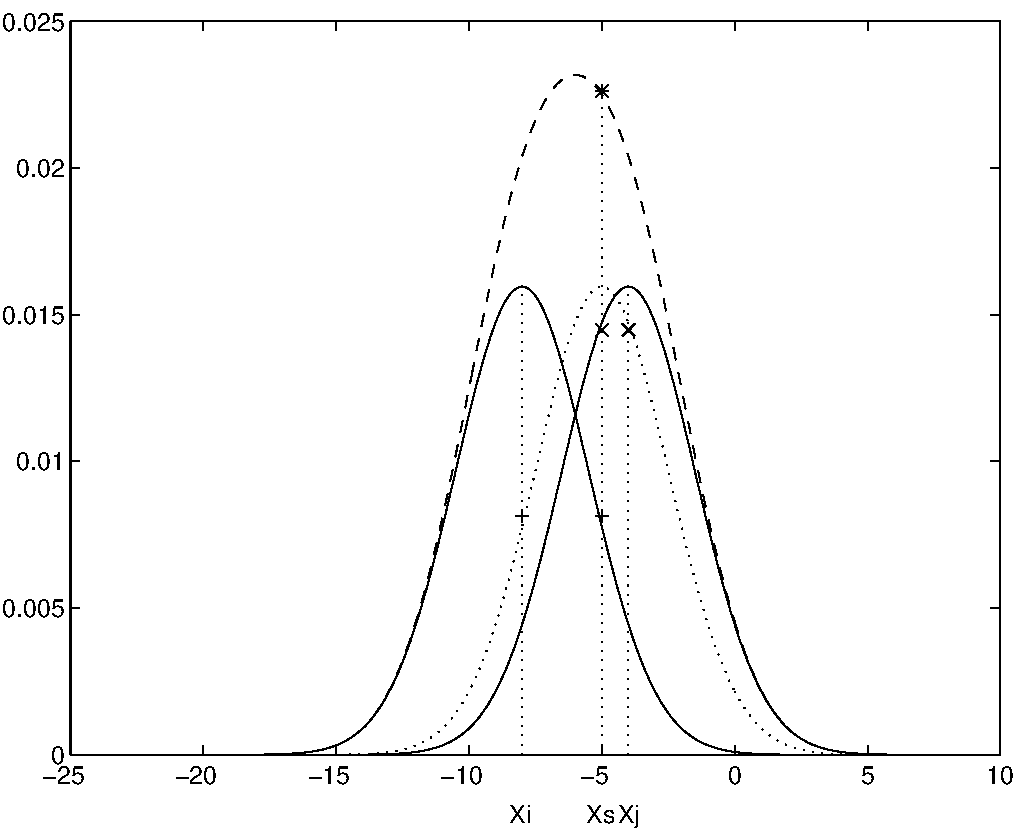
\includegraphics[height=6.5cm]{eijkel2}
%   \caption{One kernel at $x_s$ (\emph{dotted kernel}) or two kernels at $x_i$ and $x_j$ (\emph{left and right}) lead to the same summed estimate at $x_s$.
%     This shows a figure consisting of different types of lines.
%     Elements of the figure described in the caption should be set in italics, in parentheses, as shown in this sample caption. 
%     The last sentence of a figure caption should generally end with a full stop, except when the caption is not a full sentence.
%   }
%   \label{fig:example}
% \end{figure}

% \begin{figure}[tb]
%   \centering
%   \begin{subfigure}{0.68\linewidth}
%     \fbox{\rule{0pt}{0.5in} \rule{.9\linewidth}{0pt}}
%     \caption{An example of a subfigure}
%     \label{fig:short-a}
%   \end{subfigure}
%   \hfill
%   \begin{subfigure}{0.28\linewidth}
%     \fbox{\rule{0pt}{0.5in} \rule{.9\linewidth}{0pt}}
%     \caption{Another example of a subfigure}
%     \label{fig:short-b}
%   \end{subfigure}
%   \caption{Centered, short example caption}
%   \label{fig:short}
% \end{figure}

% If possible (\eg, if you use \LaTeX) please define figures as floating objects. 
% \LaTeX{} users, please avoid using the location parameter ``h'' for ``here''. 
% If you have to insert a pagebreak before a figure, please ensure that the previous page is completely filled.


% \subsection{Formulas}
% Displayed equations or formulas are centered and set on a separate line (with an extra line or half line space above and below). 
% Equations should be numbered for reference. 
% The numbers should be consecutive within the contribution, with numbers enclosed in parentheses and set on the right margin.
% For example,
% \begin{align}
%   \psi (u) & = \int_{0}^{T} \left[\frac{1}{2}
%   \left(\Lambda_{0}^{-1} u,u\right) + N^{\ast} (-u)\right] \text{d}t \; \\
% & = 0
% \end{align}
% and 
% \begin{equation}
%   E = m\cdot c^2.
%   \label{eq:important}
% \end{equation}
% Please do not include section counters in the numbering.

% Numbering equations makes reviewing more efficient, because reviewers can refer to a line on a page.  
% It is important for readers to be able to refer to any particular equation.
% Just because you did not refer to it in the text does not mean some future reader might not need to refer to it.
% It is cumbersome to have to use circumlocutions like ``the equation second from the top of page 3''.
% (Note that the ruler will not be present in the final copy, so is not an alternative to equation numbers).
% All authors will benefit from reading Mermin's description of how to write mathematics:
% \url{https://doi.org/10.1063/1.2811173}.

% % No color equations in Springer publications.
% Equations should never be in color and should be punctuated in the same way as ordinary text.
% They should not be pasted in as figures.


% \subsubsection{Lemmas, Propositions, and Theorems.}
% The numbers accorded to lemmas, propositions, and theorems, \etc should appear in consecutive order, starting with Lemma 1. 
% Please do not include section counters in the numbering like ``Theorem 1.1''.


% \subsection{Footnotes.}
% The superscript numeral used to refer to a footnote appears in the text either directly after the word to be discussed or -- in relation to a phrase or a sentence -- following the punctuation mark (comma, semicolon, or period).%
% \footnote{The footnote numeral is set flush left and the text follows with the usual word spacing. 
%   Second and subsequent lines are indented. 
% }
% For remarks pertaining to the title or the authors' names, in the header of a paper, symbols should be used instead of a number.
% Please note that no footnotes may be included in the abstract.


% \subsection{Cross References}
% For the benefit of author(s) and readers, please use the
% \begin{verbatim}
%   \cref{...}
% \end{verbatim}
% command for cross-referencing to figures, tables, equations, or sections.
% This will automatically insert the appropriate label alongside the cross reference as in this example:
% \begin{quotation}
%   To see how our method outperforms previous work, please see \cref{fig:example} and \cref{tab:headings}.
%   It is also possible to refer to multiple targets as once, \eg~to \cref{fig:example,fig:short-a}.
%   You may also return to \cref{sec:intro} or look at \cref{eq:important}.
% \end{quotation}
% If you do not wish to abbreviate the label, for example at the beginning of the sentence, you can use the
% \begin{verbatim}
%   \Cref{...}
% \end{verbatim}
% command. Here is an example:
% \begin{quotation}
%   \Cref{fig:example} is also quite important.
% \end{quotation}


% \subsection{Program Code}
% Program listings or program commands in the text are normally set in typewriter font (\eg, \texttt{printf("Hello world!\textbackslash{}n");}).


% \subsection{Citations}
% Arabic numbers are used for citation, which is sequential either by order of citation or by alphabetical order of the references, depending on which sequence is used in the list of references. 
% The reference numbers are given in brackets and are not superscript.
% Please observe the following guidelines:
% \begin{itemize}
% \item Single citation: \cite{Authors14}
% \item Multiple citation: \cite{Alpher02,Alpher03,Alpher05,Authors14b,Authors14}. 
%   The numbers should be listed in numerical order.
%   If you use the template as advised, this will be taken care of automatically.
% \item If an author's name is used in the text: Alpher \cite{Alpher02} was the first \ldots
% \end{itemize}
% Please write all references using the Latin alphabet. If the title of the book you are referring to is, \eg, in Russian or Chinese, then please write (in Russian) or (in Chinese) at the end of the transcript or translation of the title.
% All references cited in the text should be in the list of references and vice versa.

% References should be formatted with the official LNCS reference style.
% The \LaTeX{} template already takes care of that through the use of the \texttt{splncs04.bst} Bib\TeX{} style file.
% Springer strongly encourages you to include DOIs (Digital Object Identifiers) in your references (\cf \cite{ECCV2022}). 
% The DOI is a unique code allotted by the publisher to each online paper or journal article. 
% It provides a stable way of finding published papers and their metadata. 
% The insertion of DOIs increases the overall length of the references section, but this should not concern you as the reference section is not counted toward the page limit.


% \subsection{Miscellaneous}
% Compare the following:
% \begin{center}
%   \begin{tabular}{ll}
%     \verb'$conf_a$'          & $\qquad conf_a$ \\
%     \verb'$\mathit{conf}_a$' & $\qquad \mathit{conf}_a$
%   \end{tabular}
% \end{center}
% See The \TeX book, p.\ 165.

% The space after \eg, meaning ``for example'', should not be a sentence-ending space.
% So \eg is correct, \emph{e.g.} is not.
% The provided \verb'\eg' macro takes care of this.

% When citing a multi-author paper, you may save space by using ``et alia'', 
% shortened to ``\etal'' (not ``{\em et.\ al.}'' as ``{\em et\hskip 0.1em}'' is a complete word).
% If you use the \verb'\etal' macro provided, then you need not worry about double periods when used at the end of a sentence as in Alpher \etal.
% However, use it only when there are three or more authors.
% Thus, the following is correct:
%    ``Frobnication has been trendy lately.
%    It was introduced by Alpher~\cite{Alpher02}, and subsequently developed by
%    Alpher and Fotheringham-Smythe~\cite{Alpher03}, and Alpher \etal~\cite{Alpher04}.''

% This is incorrect: ``... subsequently developed by Alpher \etal~\cite{Alpher03} ...'' because reference~\cite{Alpher03} has just two authors.


% \section{Camera-Ready Manuscript Preparation}
% \label{sec:manuscript}
% This information will follow after paper decisions have been announced.


% \section{Conclusion}
% The paper ends with a conclusion. 

% \clearpage\mbox{}Page \thepage\ of the manuscript.
% \clearpage\mbox{}Page \thepage\ of the manuscript.
% \clearpage\mbox{}Page \thepage\ of the manuscript.
% \clearpage\mbox{}Page \thepage\ of the manuscript.
% \clearpage\mbox{}Page \thepage\ of the manuscript. This is the last page.
% \par\vfill\par
% Now we have reached the maximum length of an ECCV \ECCVyear{} submission (excluding references).
% References should start immediately after the main text, but can continue past p.\ 14 if needed.
% \clearpage  % TODO REVIEW/FINAL: This \clearpage needs to be removed from both review and camera-ready versions.


% % ---- Bibliography ----
% %
% % BibTeX users should specify bibliography style 'splncs04'.
% % References will then be sorted and formatted in the correct style.
% %
\bibliographystyle{splncs04}
\bibliography{egbib}
\end{document}
